\section{Introduction}
\label{sec:introduction}

\par The main objective of this laboratory assignment is to produce an audio amplifier, choosing the architecture of the Gain and Output Stages, in order to obtain the best relationship possible between the cost of the circuit and the obtained resuts. The merit of the circuit is given by:

\begin{equation}
  M = \frac {Voltage Gain * Bandwidth}{cost * Lower Cutofff Freq}.
  \label{eq:merit}
\end{equation}


\par The circuit used to produce the audio amplifier is shown in Figure\ref{fig:circuit}.

\begin{figure}[h] \centering
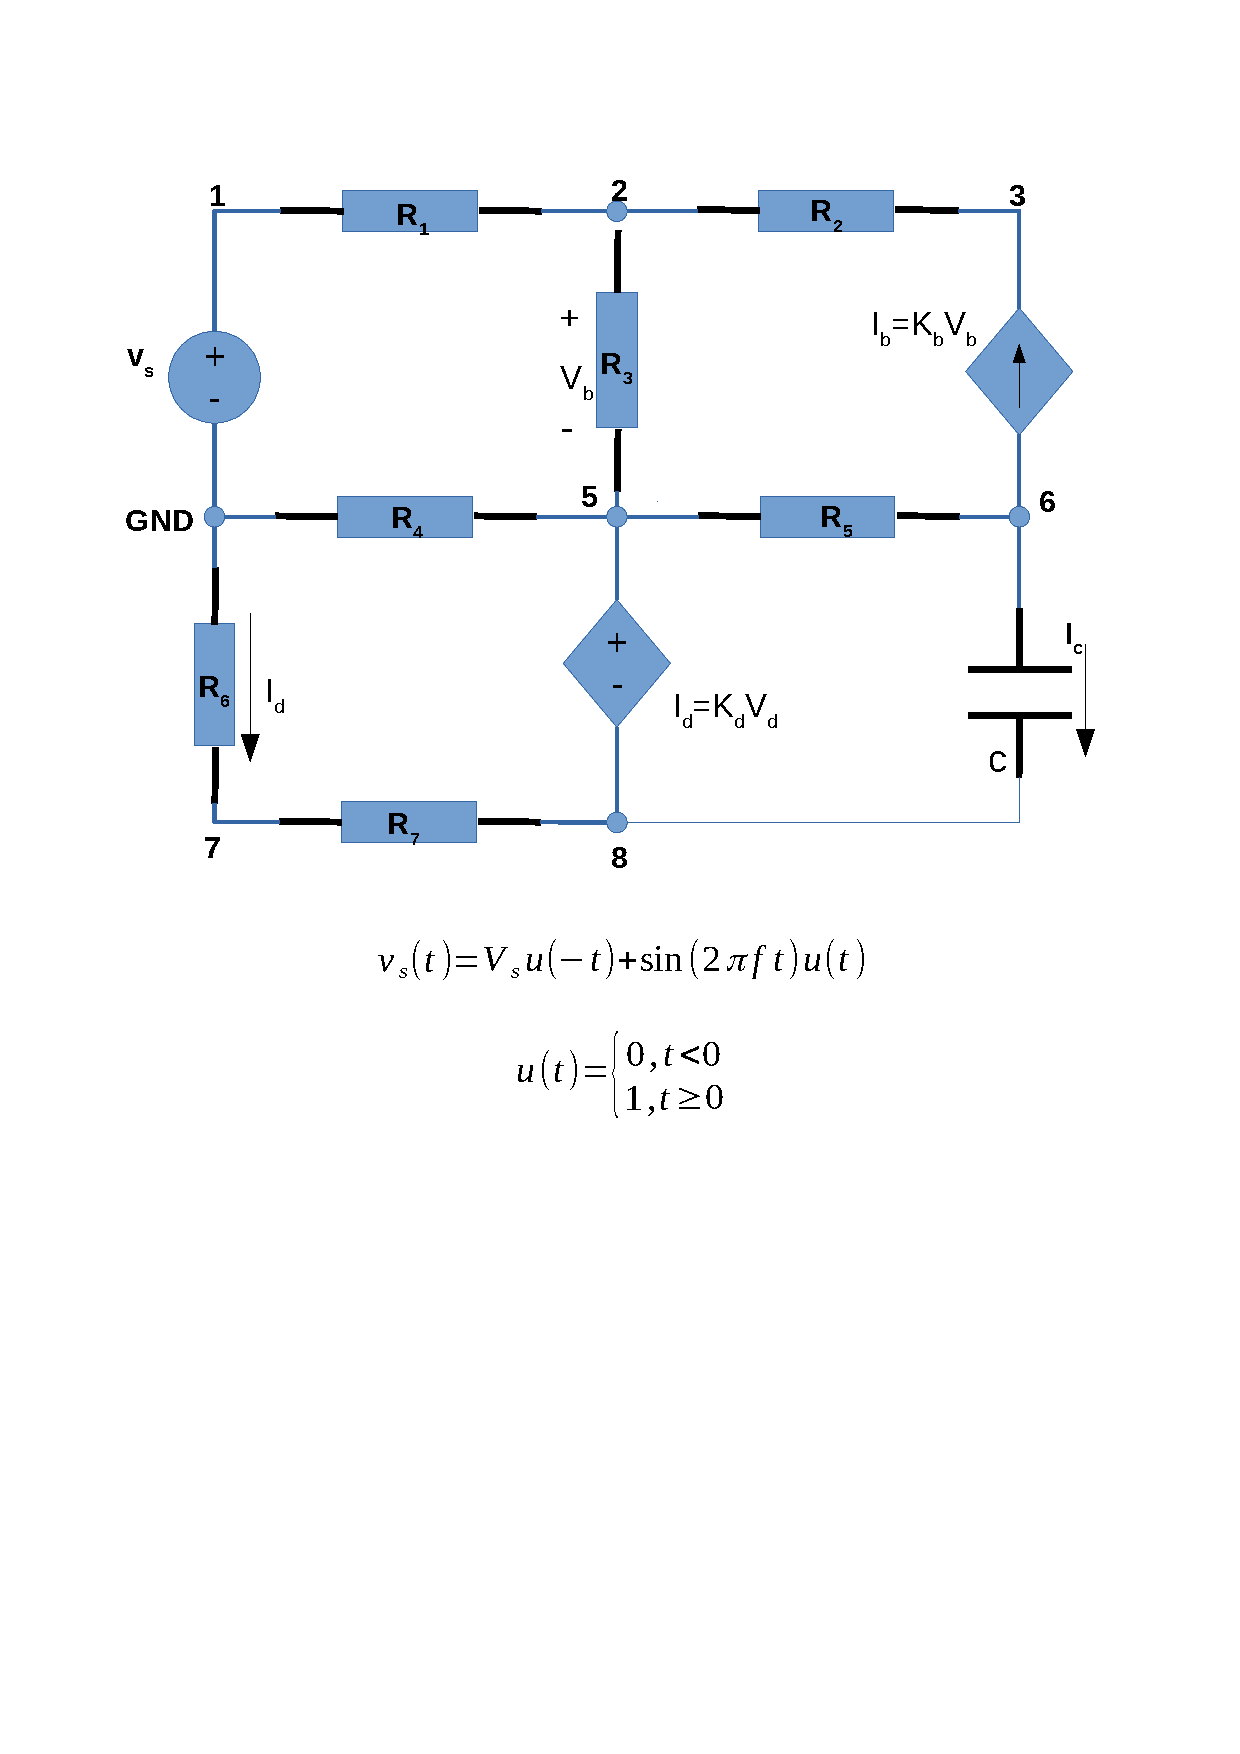
\includegraphics[width=0.6\linewidth]{circuit.pdf}
\caption{Circuit under analysis.}
\label{fig:circuit}
\end{figure}


\par In the next section (~\ref{sec:analysis}), we briefly explain the procedure to analyse theoretically the circuit above with the use of Octave maths tool. In Section 3 a simulation analysis is given, where we resorted to Ngspice to simulate the circuit, and a few graphics are presented to understand the results. The report finishes with its conclusion in section~\ref{sec:conclusion}, where we analyse side by side the theoretical and simulated results and resume the most important points of the lab assignment.

\newpage
